\nadpis{Šablona a~formální požadavky APP}
Kompletní požadavky k~absolventským písemným pracím shrnuje směrnice
Konzervatoře Pardubice č.~5/19, jejíž plné znění je k~dispozici na webových
stránkách školy v~nabídce \textit{Studium – Absolutorium}. Šablona si klade
za~cíl zjednodušit formální stránku práce, aby měli autoři více času na samotný
obsah.

\podnadpis{Doporučená minimální struktura práce}
Základní struktura absolventské práce udává zejména závazné pořadí nečíslovaných
oddílů a kapitol, které se nacházejí mimo vlastní text práce. Mezi základní
požadované prvky patří \textit{Titulní strana}, \textit{Prohlášení
o~samostatnosti}, \textit{Obsah}, \textit{Úvod}, vlastní text práce,
\textit{Závěr}, \textit{Shrnutí}, \textit{Shrnutí v~cizím jazyce},
\textit{Seznam literatury} a~přílohy.\footnote{Všechny zmíněné části jsou
v~předkládaných šablonách již předpřipraveny}

\begin{figure}[!ht]
	\begin{center}
		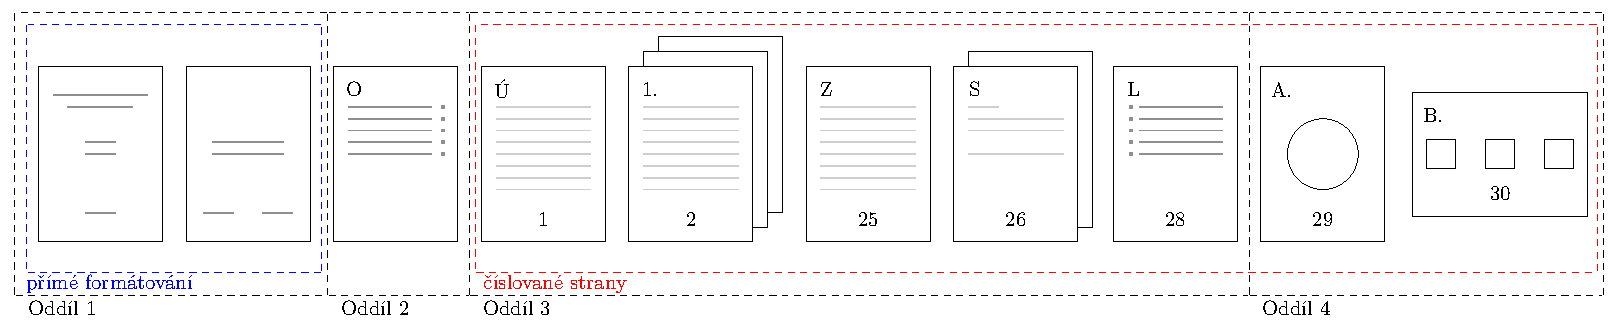
\includegraphics[width=\textwidth]{./obrazky/diagram-app.pdf}
    \end{center}

	\caption{Struktura práce}
\end{figure}

\podnadpis{Rozsah práce}
Minimálním rozsahem práce se rozumí nejnižší možný počet stran vlastního textu,
obvykle od~\textit{Úvodu} po konec \textit{Závěru}, udávaný v~normostranách.
Pojem normostrana je definován jako strojopis 30 řádků po 60 úhozech, tedy
přesně 1\,800 znaků včetně mezer. Šablony jsou koncipovány tak, aby v~nich psaná
jedna strana A4 odpovídala přibližně 1\,400~–~2\,400 úhozům, což je přibližně
v~rozsahu ±30~\% normostrany.

Do rozsahu vlastního textu se dále také počítají textové přílohy, ale pouze
jsou-li autorským dílem (např.~provedené rozhovory). V~této ukázce je jako
příklad první přílohy přepis korespondence, který autorským dílem \textit{není}.

\noindent
Pro APP je minimální hranicí 20 stran textu, samozřejmě je lépe, je-li stran
napsáno více, optimum bude cca na 22-25 tiskových stranách. Horní hranici je
nutné konzultovat s~vedoucím práce, rozsah by však neměl být zbytečně objemný.

\podnadpis{Formální úprava}
Požadavky na formální úpravu zahrnují především vzhled stránky, vše je již
obsaženo v této šabloně. Zejména se jedná o~formát papíru A4, okraje stránky
po 2,5~cm shora, zespodu a~zprava, levý okraj 4~cm.  Formální úprava dále
specifikuje velikost písma a~proklad řádkování vlastního textu, způsob číslování
a~umístění kapitol, stránek a~příloh.

\podnadpis{Forma odevzdání}
Práce se odevzdává výhradně ve~formátu PDF (Portable Document Format). PDF
soubor \texttt{app.pdf} vznikne automaticky překladem v~prostředí \XeLaTeX
jednoduchým zavoláním \texttt{make}.

% ------------------------------------------------------------------------------
\nadpis{Nadpis první úrovně}
Číslovaný nadpis první úrovně lze realizovat příkazem
\texttt{{\textbackslash}nadpis\{Text nadpisu\}}. První úroveň nadpisu otevírá
každou hlavní \emph{kapitolu} práce se~samostatným tematickým celkem a~vždy
začíná na~nové stránce. Nadpis hlavní kapitoly nikdy nemůže okamžitě navazovat
na~dílčí podnadpisy, musí za~ním stát krátký odstavec stručně charakterizující
další obsah.

\podnadpis{Nadpis druhé úrovně}
Číslovaný nadpis druhé úrovně je k~dispozici pod~příkazem
\texttt{{\textbackslash}podnadpis\{Text podnadpisu\}}. Druhá úroveň člení každou
kapitolu na~její stěžejní body a~obvykle se zde nachází nejvíce odstavců textu.

První řádek každého následujícího odstavce je automaticky odsazen. Je třeba
dávat pozor na~místa, kde je automatické odsazení nežádoucí -- pokud
by odstavec začínal na~nové straně a~po~vloženém obrázku nebo tabulce.

\podpodnadpis{Nadpis třetí úrovně}
Nadpis třetí úrovně je uveden příkazem
\texttt{{\textbackslash}podpodnadpis\{Text podpodnadpisu\}}. Závěrečné práce by
neměly přesáhnout tři úrovně členění textu a~třetí úroveň je obecně vhodné
věnovat pro~popisy konkrétních případů, které obecně zahrnuje nadpis druhé
úrovně (př.~\textit{1 - Hudba}, \textit{2 - Hudební nástroje}, \textit{3 -
Smyčcové nástroje}).

\podnadpis{Bibliografické citace}

Šablona předpokládá používání zdrojů zapsaných ve~stylu \hologo{BibTeX}
v~externím souboru \texttt{literatura.bib}, který je při automatické kompilaci
překládán nástrojem \texttt{biber}. V~ukázce jsou pro~příklad uvedeny časté typy
zdrojů (kniha, akademická práce, elektronický článek, elektronický zdroj) tak,
aby odpovídaly normě ČSN~ISO~690 (01~0197) podle znění platného od~1.~dubna
2011. Preferovanou citační metodou je \emph{vacouverský stylem číselných odkazů}
v~hranatých závorkách:~\cite[19]{hladena19}.

\nocite{*}

\podnadpis{Jiné funkce a~objekty}
Lze psát technické tóny \nota{Eb2} (\texttt{{\textbackslash}nota\{Eb2\}}),
nebo \nota{C#6} (\texttt{{\textbackslash}nota\{C\#6\}}). Dále je také
pro matematické výsledky k~dispozici \doubleunderline{dvojité podržení}
(\texttt{{\textbackslash}doubleunderline\{\}}) a~vedle obyčejných českých
uvozovek (\texttt{{\textbackslash}uv\{\}}) také \juv{jednoduché uvozovky}
(\texttt{{\textbackslash}juv\{\}}), které jsou vhodné pro~zahrnutí přímé řeči
v~přímé řeči.

Vkládání obrázků není nijak omezeno, řídí se pouze obecnými pravidly --
k~použití jsou vhodné zejména vektorové formáty (PDF), obrázek by neměl být
větší než třetina výšky tiskové strany (v~tom případě patří do~příloh,
viz~ukázka v~příloze~\ref{priloha:partitura}), každý obrázek by měl mít svůj
popisek a~musí být v~předcházejícím odstavci alespoň stručně uveden: Následující
obrázek zachycuje logo školy.

\begin{figure}[!ht]
	\begin{center}
		
\includegraphics[width=60mm]{./obrazky/kp-logo.pdf}
    \end{center}

	\caption{Logo: Konzervatoř Pardubice}
\end{figure}

\noindent
Odstavec ihned za~obrázkem není na~svém prvním řádku odsazen
(\texttt{{\textbackslash}noindent}) a~může zahrnovat podrobnější rozbor jeho
obsahu.
